%
% helmholtz.tex -- Geht auf die Helmholtzschen Wirbelsätze ein
%
% !TEX root = ../../buch.tex
% !TEX encoding = UTF-8
%
\section{Helmholtzsche Wirbelsätze}
\kopfrechts{Helmholtzsche Wirbelsätze}%
Um das Verhalten von Wirbelringen besser zu verstehen, sind die sogenannten helmholtzschen Wirbelsätze sehr nützlich. 
Mitte 19. Jahrhundert formulierte der deutsche Physiker Hermann von Helmholtz drei Wirbelsätze und veröffentlichte diese im Journal für die reine und angewandte Mathematik \cite{Wirbelringe:JournalHelmholtz}.
\index{Wirbelsätze}%
\index{Helmholtz, Hermann von}%
In seinem veröffentlichten Paper definiert er auch die Begriffe Wirbellinie und Wirbelfaden, welche wir bereits kennen.

\subsection{Wirbelsätze}

\begin{figure}
    \centering
    \subfigure[1. Wirbelsatz \label{Wirbelringe:fig:Helmholtz_1}]{
        \includegraphics[width=0.3\textwidth]{papers/wirbelringe/fig/cube_still_particles.pdf}
    }\hfill
    \subfigure[2. Wirbelsatz \label{Wirbelringe:fig:Helmholtz_2}]{
        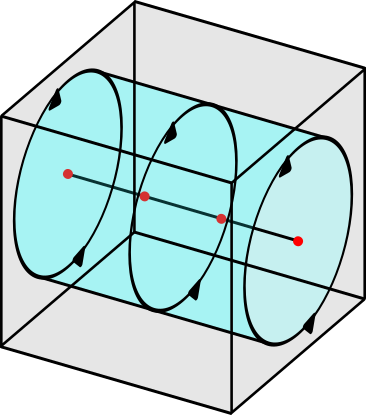
\includegraphics[width=0.3\textwidth]{papers/wirbelringe/fig/cube_still_particles_rotation.pdf}
    }\hfill
    \subfigure[3. Wirbelsatz \label{Wirbelringe:fig:Helmholtz_3}]{
        \includegraphics[width=0.3\textwidth]{papers/wirbelringe/fig/cube_constant_rotation.pdf}
    }
    \caption{Helmholtzsche Wirbelsätze visuell dargestellt in einem abgeschlossenen System mit idealen Grenzflächen.}
    \label{Wirbelringe:fig:Wirbelsaetze}
\end{figure}

\begin{satz}[Erster Wirbelsatz]
    \label{Wirbelringe:satz:wirbelsatz1}
    In Abwesenheit von wirbelanfachenden äusseren Kräften bleiben wirbelfreie Strömungsgebiete wirbelfrei.
\end{satz}

Anders gesagt, Teilchen die ruhen, bleiben in Ruhe. 
Siehe Abbildung \ref{Wirbelringe:fig:Helmholtz_1}: 
Alle Teilchen in Rot bewegen sich nicht, da der Betrachtungsraum abgeschlossen ist und diese {\em nicht} Teil eines Wirbels sind.

\begin{satz}[Zweiter Wirbelsatz]
    \label{Wirbelringe:satz:wirbelsatz2}
    Fluidelemente, die auf einer Wirbellinie liegen, verbleiben auf dieser Wirbellinie.
\end{satz}

Dies gilt auch, wenn sich diese Wirbellinie fortbewegt.
Allerdings heisst das nicht, dass Teilchen, die sich nicht von Anfang an auf einer Wirbellinie befinden, dort nicht mehr hingelangen können.
Siehe Abbildung \ref{Wirbelringe:fig:Helmholtz_2}:
Alle in Rot dargestellten Teilchen bewegen sich nicht, da sich die Wirbellinie (relativ zum Beobachtungsraum) nicht bewegt und sie auf der Wirbellinie liegen.

Um den nächsten Wirbelsatz zu verstehen, müssen wir zunächst die Zirkulation einführen.
\index{Zirkulation}%
Die \emph{Zirkulation} mit dem Formelzeichen \(\Gamma\) sagt aus, wie stark die Teilchen in einem Wirbelring rotieren.
Die Zirkulation ist definiert als 
\begin{equation}
    \label{Wirbelringe:eq:Zirkulation}
    \Gamma
    = 
    \oint_{c} \vec{u} \cdot d \vec{l},
\end{equation}
wobei \(c\) die Kontur des jeweiligen Flächenstücks, in dem der Wirbel liegt, ist und \(\vec{u}\) die Geschwindigkeit der rotierenden Partikel.

\begin{satz}[Dritter Wirbelsatz]
    \label{Wirbelringe:satz:wirbelsatz3}
    Die Zirkulation entlang eines Wirbelfadens ist konstant. 
\end{satz}

Somit kann man die Zirkulation an einer Stelle des Wirbelrings bestimmen und kennt die Zirkulation des ganzen Rings.
Siehe Abbildung \ref{Wirbelringe:fig:Helmholtz_3}: 
Die Zirkulation, dargestellt als Grösse der Pfeile, ist bei allen drei dargestellten Konturen des Wirbelfadens gleich gross.

\subsection{Zusammenhang von der Zirkulation und Wirbelstärke\label{Wirbelringe:Stokes}}

Die Zirkulation \(\Gamma\) kann auch anders beschrieben werden. 
In der Einleitung wurde erwähnt, dass Wirbel eine Wirbelstärke \(\vec{\omega}\) besitzen.
Diese ist definiert als
\[
\vec{\omega}
=
\operatorname{rot}(\vec{u})
\]
und beschreibt wie schnell sich ein Wirbel an einem beliebigen Punkt dreht.
Integriert man \(\vec{\omega}\) über eine Fläche \(S\) mit Rand \(c\), erhält man nach dem Satz von Stokes (Satz \ref{buch:green:green:satz:stokes})
\begin{align*}
\iint_{S} \vec{\omega} \cdot d \vec{S}
&=
\iint_{S} \operatorname{rot}(\vec{u})\cdot  d \vec{S}\\
&=
\int_{\partial S = c} \vec{u} \cdot d\vec{l},
\end{align*}
also die Zirkulation.

\subsection{Verhalten an Grenzflächen\label{Wirbelringe:Grenzflaechen}}

Mit den vorhergegangenen Regeln kann das Verhalten von Wirbelringen nun einfacher nachvollzogen werden.
Allerdings haben wir Grenzflächen noch nicht betrachtet.
\index{Grenzfläche}%
Diese sind wichtig, da in der Realität immer solche Grenzflächen vorhanden sind.
Grenzflächen entstehen immer dort, wo es Materialübergänge gibt oder am Rand des Betrachtungsraums.

Aus der Identität der Quellenfreiheit von Wirbeln (Gleichung \eqref{Wirbelringe:eq:wIdent}) lässt sich schliessen, dass Teilchen in einem Wirbelring Grenzflächen nicht durchqueren.
Allerdings können Wirbellinien darauf enden, da die Teilchen zwar auf der Grenzfläche sind, diese aber nicht überschreiten.
Dies macht auch dann Sinn, wenn eine Wirbellinie als Kreis geschlossen ist, da sonst Satz \ref{Wirbelringe:satz:wirbelsatz3} verletzt wird.

Was man allerdings nicht vergessen sollte ist, dass bei Grenzflächen, welche durch Materialübergänge entstehen, die Teilchen diese Grenzfläche nicht überschreiten können.
Zum Beispiel kann sich ein Wirbel im Wasser nicht auf die angrenzende Wand ausdehnen.
Die Wirbellinie endet auf der Wand.
